\documentclass[notes]{subfiles}
\begin{document}
	\addcontentsline{toc}{section}{1.2 - Mathematical Models: A Catalog of Essential Functions}
	\refstepcounter{section}
	\fancyhead[RO,LE]{\bfseries \nameref{cs12}} 
	\fancyhead[LO,RE]{\bfseries \small \currentname}
	\fancyfoot[C]{{}}
	\fancyfoot[RO,LE]{\large \thepage}	%Footer on Right \thepage is pagenumber
	\fancyfoot[LO,RE]{\large Chapter 1.2}
	
\section*{Mathematical Models: A Catalog of Essential Functions}\label{cs12}
	\subsection*{Before Class}
	\addcontentsline{toc}{subsection}{Before Class}
	\subsubsection*{Linear Functions}
	\addcontentsline{toc}{subsubsection}{Linear Functions}
		Remember that a linear function requires two pieces of information- a starting value ($b$, the $y$-intercept), and an amount of incremental change in the independent variable ($m$, the slope of the function).  This gives us three ways to describe a linear function:\\[10pt]
		\showto{ins}{
			\begin{itemize}
				\item \underline{Verbally}: \fbox{A function with a constant rate of change}
				\item \underline{Graphically}: \fbox{They are lines...}
				\item \underline{Algebraically}: \fbox{$f(x) = mx + b$}
			\end{itemize}
		}
		\showto{st}{
			\begin{itemize}
				\setlength\itemsep{25pt}
				\item \underline{Verbally}:
				\item \underline{Graphically}: \\[1.5in]
				\item \underline{Algebraically}: 
			\end{itemize}
		}
			\vs{1}
	
		\begin{question}
			Given two points $(x_1,y_1)$ and $(x_2,y_2)$, how can we find the slope of the line between them?
		\end{question}
			\vs{1}
			\newpage
			
		\begin{ex}
			The following table gives the percentage of new companies which remained open $t$ years after beginning business.
			\begin{center} 
				{\renewcommand{\arraystretch}{1.2}
				\begin{tabular}{|l||c|c|c|c|c|c|} \hline
					\textbf{Years After Opening} & 5 & 6 & 7 & 8 & 9 & 10\\ \hline
					\textbf{Companies Still Open} (in \%) & 50 & 47 & 44 & 41 & 38 & 35\\ \hline
				\end{tabular}
				}
			\end{center}
			\begin{enumerate}[(a)]
				\item Plot the points on the graph below
					\begin{center} 
						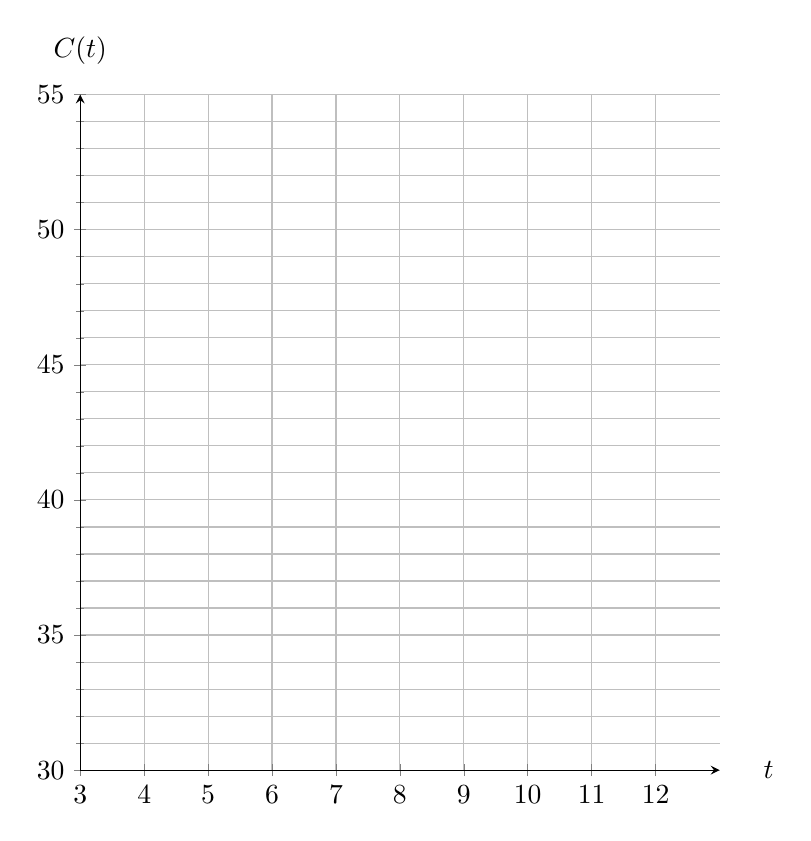
\begin{tikzpicture}
							\begin{axis}[
								width = .8\textwidth,
								height = 4in,
								grid = both,
								axis x line = bottom,
		    						axis y line = left,
			    					every axis y label/.style={at={(ticklabel cs:1.1)}},
									y label style={at={(axis description cs:.0,1.1)},anchor=north},
			    					ylabel = {$C(t)$},
		    						every axis x label/.style= {at ={(ticklabel cs:1)}},
		    							x label style={at={(axis description cs:1.1,0)},anchor=east},
		    						xlabel = {$t$},
								xmin=3, xmax = 13,
									xtick = {3,4,...,12},
		       			    		ymin=30, ymax = 55,
		       			    			minor y tick num = 4,
							]
							\end{axis}

						\end{tikzpicture}
					\end{center}
					
				\item Use the data to find an equation for the line between these points.
					\vs{2}
					
				\item Give an interpretation for the slope of $C(t)$
					\vs{1}
					
			\end{enumerate}
		\end{ex}
			\newpage
			
	\subsubsection*{Polynomials}
	\addcontentsline{toc}{subsubsection}{Polynomials}
		\begin{defn}[Polynomial]
			A function $P$ is called a \textbf{polynomial} if 
			\showto{ins}{
				\[P(x) = a_nx^n + a_{n-1}x^{n-1}+ \cdots + a_2x^2 + a_1x + a_0\]			
				where $n$ is a nonnegative integer and the numbers $a_i$ are constants called the \emph{coefficients} of the polynomial.  The \emph{degree} of the polynomial is the power of the leading coefficient.
			}
			\showto{st}{\\ \vspace{.5in}
				where $n$ is \blank{3} and the numbers $a_i$ are constants, called \\ \vspace{15pt} \blank{2}.  The \emph{degree} of the polynomial is  \blank{2} \\ \vspace{15pt} \blank {3.5}.
			}
		\end{defn}
		
 		\showto{ins}{
 		\begin{flushleft}
	 		\tabulinesep = 2mm	 	
	 		\setlength{\arrayrulewidth}{1.5pt}	
	 		\begin{tabu}{| X[.5,c] | X[.75,c] | X[c] | X[c] |}\hline 
	 			\multicolumn{4}{|c|}{{\large \textbf{Common Polynomials}}} \\ \hline
	 			
	 			\textbf{Polynomial} 	& \textbf{Equation}	& \textbf{Graph} ($a_n > 0$)	& \textbf{Graph} ($a_n < 0$) \\ \hline 
				Linear				& $a_1x + a_0$ & 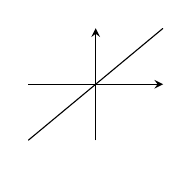
\begin{tikzpicture}\begin{axis}[scale = .25, axis x line = middle, axis y line = middle, ticks = none] \addplot[domain = -1:1] {x}; \end{axis} \end{tikzpicture} & 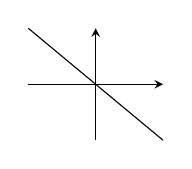
\begin{tikzpicture}\begin{axis}[scale = .25, axis x line = middle, axis y line = middle, ticks = none] \addplot[domain = -1:1] {-1*x}; \end{axis} \end{tikzpicture} \\ \hline
				
				Quadratic			& $a_2x^2 + a_1x + a_0$	& 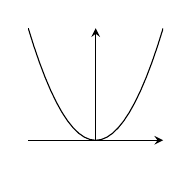
\begin{tikzpicture}\begin{axis}[scale = .25, axis x line = middle, axis y line = middle, ticks = none] \addplot[domain = -1:1] {x^2}; \end{axis} \end{tikzpicture} & 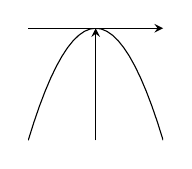
\begin{tikzpicture}\begin{axis}[scale = .25, axis x line = center, axis y line = middle, ticks = none] \addplot[domain = -1:1] {-1*x^2}; \end{axis} \end{tikzpicture} \\ \hline
		 		
		 		Cubic				& $a_3x^3 + a_2x^2 + a_1x + a_0$	& 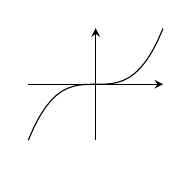
\begin{tikzpicture}\begin{axis}[scale = .25, axis x line = middle, axis y line = middle, ticks = none] \addplot[domain = -1:1] {x^3}; \end{axis} \end{tikzpicture} & 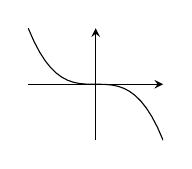
\begin{tikzpicture}\begin{axis}[scale = .25, axis x line = middle, axis y line = middle, ticks = none] \addplot[domain = -1:1] {-1*x^3}; \end{axis} \end{tikzpicture} \\ \hline
		 		
		 		Even Degree			& \makecell{$a_nx^n + \cdots a_1x + a_0$ \\ $n$ even}	& 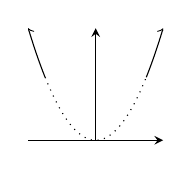
\begin{tikzpicture}\begin{axis}[scale = .25, axis x line = middle, axis y line = middle, ticks = none] \addplot[<-,domain = -1:-.75] {x^2}; \addplot[domain = -.75:.75, dotted] {x^2}; \addplot[domain = .75:1,->] {x^2}; \end{axis} \end{tikzpicture} & 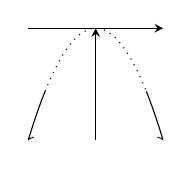
\begin{tikzpicture}\begin{axis}[scale = .25, axis x line = middle, axis y line = middle, ticks = none] \addplot[<-,domain = -1:-.75] {-1*x^2}; \addplot[domain = -.75:.75, dotted] {-1*x^2}; \addplot[domain = .75:1,->] {-1*x^2}; \end{axis} \end{tikzpicture} \\ \hline
		 		
		 		Odd Degree			& \makecell{$a_nx^n + \cdots a_1x + a_0$ \\ $n$ odd}	& \begin{tikzpicture}\begin{axis}[scale = .25, axis x line = middle, axis y line = middle, ticks = none] \addplot[<-,domain = -1:-.75] {x^3}; \addplot[domain = -.75:.75, dotted] {x^3}; \addplot[domain = .75:1,->] {x^3}; \end{axis} \end{tikzpicture} & \begin{tikzpicture}\begin{axis}[scale = .25, axis x line = middle, axis y line = middle, ticks = none] \addplot[<-,domain = -1:-.75] {-1*x^3}; \addplot[domain = -.75:.75, dotted] {-1*x^3}; \addplot[domain = .75:1,->] {-1*x^3}; \end{axis} \end{tikzpicture} \\ \hline
		 	\end{tabu}
	 	\end{flushleft}
	 	}
	 	\showto{st}{
	 	\begin{flushleft}
	 		\tabulinesep = 2mm	 	
	 		\setlength{\arrayrulewidth}{1.5pt}	
	 		\begin{tabu}{| X[.5,c] | X[1,c] | X[c] | X[c] |}\hline 
	 			\multicolumn{4}{|c|}{{\large \textbf{Common Polynomials}}} \\ \hline
	 			
	 			\textbf{Polynomial} 	& \textbf{Equation}	& \textbf{Graph} ($a_n > 0$)	& \textbf{Graph} ($a_n < 0$) \\ \hline 
	 								& & & \\
				Linear				& & &  \\ 
									& & &  \\
									& & & \\ \hline
									& & & \\
				Quadratic			& & &  \\ 
									& & &  \\
		 							& & & \\ \hline
		 							& & & \\
		 		Cubic				& & & \\ 
		 							& & &  \\
		 							& & & \\ \hline
		 							& & & \\
		 		Even Degree			& & & \\ 
		 							& & &  \\
		 							& & & \\ \hline
		 							& & & \\
		 		Odd Degree			& & & \\ 
		 							& & &  \\
		 							& & & \\ \hline
		 	\end{tabu}
	 	\end{flushleft}
	 	}
	 	\newpage
	 	
	 	\subsubsection*{Other Functions}
		\addcontentsline{toc}{subsubsection}{Other Functions}
		\begin{defn}[Exponential/Logarithmic Function]
			An \textbf{exponential function} is a function of the form \showto{ins}{\fbox{$f(x) = b^x$}} \showto{st}{\blank{1.5}}, where the base $b$ is a positive constant.\\ \vspace{25pt}
			
			A \textbf{logarithmic function} is a function of the form \showto{ins}{\fbox{$f(x) = \log_b x$}}\showto{st}{\blank{2}}, where the base $b$ is a positive constant.
		\end{defn}
			\vs{.25}
		Exponential and logarithmic functions have these properties:
		\showto{ins}{
			\begin{flushleft}
				\tabulinesep = 2mm
				\setlength{\arrayrulewidth}{1.5pt}
				\begin{tabu}{| X[c] | X[c] | X[c] | X[c] |}\cline{2-4}
					\multicolumn{1}{c|}{} & \textbf{Domain} & \textbf{Range} & \textbf{Asymptotes?} \\ \hline
					$f(x) = b^x$		& $(-\infty,\infty)$	& $(0,\infty)$	& $y = 0$ \\ \hline
					$g(x) = \log_b x$& $(0,\infty)$		& $(-\infty,\infty)$& $x = 0$ \\ \hline			
				\end{tabu}		
			\end{flushleft}
		}
		\showto{st}{
			\begin{flushleft}
				\tabulinesep = 2mm
				\setlength{\arrayrulewidth}{1.5pt}
				\begin{tabu}{| X[c] | X[c] | X[c] | X[c] |}\cline{2-4}
					\multicolumn{1}{c|}{} & \textbf{Domain} & \textbf{Range} & \textbf{Asymptotes?} \\ \hline
									&					&				& \\
					$f(x) = b^x$		& 					& 				&  \\ 
									&					&				& \\ \hline
									&					&				& \\
					$g(x) = \log_b (x)$	& 					& 				&  \\ 			
									&					&				& \\ \hline
				\end{tabu}
			\end{flushleft}	
		}
			\vs{.25}
			\newsec
	\subsubsection*{Pre-Class Activities}
	\addcontentsline{toc}{subsubsection}{Pre-Class Activities}
		\begin{ex}
			\begin{enumerate}[(a)]
				\item Find an equation for the family of linear functions with slope $-1$, and sketch a few members of the family.
					\vs{1}
					
				\item Find an equation for the family of linear functions such that $f(2) = 1$, and sketch a few members of the family.
					\vs{1}
					
				\item Which function belongs to both families?
					\vs{1}
			\end{enumerate}
		\end{ex}
			\newpage
			
		\begin{ex}
			Find an expression for a quadratic function $f$ if $f(-2) = 2$, $f(0) = 1$, and $f(1) = -2.5$.
		\end{ex}
			\vs{1}
			
		\begin{ex}
			The monthly cost of driving a car depends on the number of miles driven.  Casey found that in April, it cost her \$350 to drive 450 miles, and in June, it cost her \$460 to drive 800 miles.  Express your answer exactly (no decimals).
			\begin{enumerate}[(a)]
				\item Express the monthly cost $C$ as a function of the distance driven ($d$), assuming that a linear relationship gives a suitable model.
					\vs{.5}
				\item Use (a) to predict the cost of driving 1500 miles per month.
					\vs{.5}
				\item Sketch the graph of the linear function.  What does the slope represent?  Include units.
					\vs{1}
				\item What does the $C-$intercept represent?
					\vs{.5}
				\item Why does a linear function give a suitable model in this situation?
					\vs{.5}
			\end{enumerate}
		\end{ex}
	 		\newpage
	 		
	\subsection*{In-Class} 
	\addcontentsline{toc}{subsection}{In-Class}		
	\subsubsection*{Power Functions}
	\addcontentsline{toc}{subsubsection}{Power Functions}
		\begin{defn}[Power Function]
			A \textbf{power function} is any function of the form \showto{ins}{\fbox{$x^a$}}\showto{st}{\blank{2}}, where $a$ is a\\ \showto{ins}{\fbox{constant}} \showto{st}{\\ \vspace{25pt}\blank{2}}.
		\end{defn}
		
		\begin{ex}
			Describe the difference between a \emph{power function} and a \emph{polynomial}.
		\end{ex}
			\vs{1}
			
		\begin{ex}
			We will look at three special power functions.
			\begin{enumerate}[(a)]
				\item If $a$ is a positive integer, what kind of functions do we see?  Sketch a few examples.
					\vs{1}

				\item If $a = \dfrac{1}{n}$ (where $n$ is a positive integer), rewrite the power function using rules of exponents.  
					\vs{1}
					\newpage

				\item The functions in part (b) are called \blank{1.5} functions.  Sketch the graph of the power function if $a = \dfrac{1}{2}$ and $a = \dfrac{1}{3}$.  
					\vs{1}
					
					
				\item When $a=-1$, we call the power function the \blank{1.5} function.  Sketch the graph.
					\vs{1}
					
			\end{enumerate}
		\end{ex}
				
	\subsubsection*{Rational Functions}
	\addcontentsline{toc}{subsubsection}{Rational Functions}
		\begin{defn}[Rational Function]
			A \textbf{rational function} is a ratio of two polynomials, written as
			\showto{ins}{
				\[f(x) = \dfrac{P(x)}{Q(x)}\]
				where $P$ and $Q$ are polynomials. \\
			}
			\showto{st}{
				\\ \vspace{.75in}
			}
			The domain of a rational function consists of all values of $x$ such that 
			\showto{ins}{
				\fbox{$Q(x)\neq 0$}.
			}
			\showto{st}{
				\blank{1.5}.
			}
		\end{defn}
		
		\begin{ex}
			Write the domain of the following functions, in interval notation.
			\begin{enumerate}[(a)]
				\item $f(x) = \dfrac{1}{x}$
					\vs{1}
					\newpage

				\item $g(x) = \dfrac{2x^3 - 1}{x^5 + 1}$
					\vs{1}
					
				\item $h(x) = \dfrac{6x^4 + x^3 - 7x^2 + 6.5029}{x^2 - 9}$
					\vs{1}
			\end{enumerate}
		\end{ex}
			
	\subsubsection*{Algebraic Functions}
	\addcontentsline{toc}{subsubsection}{Algebraic Functions}
		\begin{defn}[Algebraic Function]
			A function $f$ is called an \textbf{algebraic function} if it can be constructed using algebraic operations such as:
			\showto{ins}{
				\fbox{addition, subtraction, multiplication, division, and taking roots}
			}
			\showto{st}{
				\\ \vspace{10pt} \blank{6.5} \\ \vspace{15pt}
			}
			starting with
			\showto{ins}{
				\fbox{polynomials}
			}
			\showto{st}{
				\blank{3}.
			}
		\end{defn}
		\newpage
		
		\begin{ex}
			Write an example of an algebraic function using at least one of each type of function we have covered so far.
		\end{ex}
			\vs{1}

	\subsubsection*{Trigonometric Functions}
	\addcontentsline{toc}{subsubsection}{Trigonometric Functions}
		\showto{ins}{
		\begin{flushleft}
			\tabulinesep = 5mm
			\setlength{\arrayrulewidth}{1.5pt}	
	 		\begin{tabu}{| X[1,c]  X[1,c]  X[1,c] | X[2,c,p] |} \hline
	 			\multicolumn{4}{|c|}{\large{\textbf{Basic Trigonometric Functions}}}\\ \hline
	 			$\sin x = \dfrac{\text{opp}}{\text{hyp}}$ & $\cos x = \dfrac{\text{adj}}{\text{hyp}}$ & $\tan x = \dfrac{\text{opp}}{\text{adj}} $	& 
	 			\multirow{3}{*}{
	 				\begin{tikzpicture}[scale = .9]
 						\coordinate (one) at (0,0);
 						\coordinate (two) at (4,3); 
 						\coordinate (three) at (4,0);
						\draw (one)--(two) node[midway, yshift = 9pt, sloped] {hyp};
						\draw (two)--(three) node[midway, xshift = 14pt, yshift = -6pt] {opp};
						\draw (three)--(one) node[midway, yshift = -9pt] {adj};
						\draw (.75,0) node[yshift = 5pt] {$x$};
					\end{tikzpicture}
					} \\ & & & \\
				$\csc x = \dfrac{\text{hyp}}{\text{opp}}$ & $\sec x = \dfrac{\text{hyp}}{\text{adj}}$ & $\cot x = \dfrac{\text{adj}}{\text{opp}}$ & \\ \hline
	 		\end{tabu}
		\end{flushleft}
		}
		\showto{st}{
		\begin{flushleft}
			\tabulinesep = 3mm
			\setlength{\arrayrulewidth}{1.5pt}	
	 		\begin{tabu}{| X[1,c]  X[1,c]  X[1,c] | X[1.5,c,p] |} \hline
	 			\multicolumn{4}{|c|}{\large{\textbf{Basic Trigonometric Functions}}}\\ \hline
	 			&&&\multirow{5}{*}{
	 				\begin{tikzpicture}[scale = .9]
 						\coordinate (one) at (0,0);
 						\coordinate (two) at (4,3); 
 						\coordinate (three) at (4,0);
						\draw (one)--(two) node[midway, yshift = 9pt, sloped] {hyp};
						\draw (two)--(three) node[midway, xshift = 14pt, yshift = -6pt] {opp};
						\draw (three)--(one) node[midway, yshift = -9pt] {adj};
						\draw (.75,0) node[yshift = 5pt] {$x$};
					\end{tikzpicture}
					} \\
	 			$\sin x = \hspace*{20pt}$ & $\cos x = \hspace*{20pt}$ & $\tan x = \hspace*{30pt} $	& \\
	 			 & & & \\
				$\csc x = \hspace*{20pt}$ & $\sec x = \hspace*{20pt} $& $\cot x = \hspace*{30pt}$ & \\ 
				&&& \\ \hline
	 		\end{tabu}
		\end{flushleft}
		}
			\vs{.5}
			
		Here are some useful properties of trigonometric functions  
		\showto{ins}{
			\begin{flushleft}
				\tabulinesep = 5mm
				\setlength{\arrayrulewidth}{1.5pt}
				\begin{tabu}{| X[c] | X[c] | X[c] | X[1.2,c] | X[c] | X[1.4,c] | X[1.4,c] | } \cline{2-7}
					\multicolumn{1}{c|}{} & $\sin x$ 		& $\cos x$ 			& $\tan x$ 											& $\cot x$ 							& $\sec x$ 											  & $\csc x$ \\ \hline
					\textbf{Domain}		& $(-\infty,\infty)$& $(-\infty,\infty)$	& \makecell{$x\neq \dfrac{\pi}{2} + \pi k$ \\ $k\in \Z$}	& \makecell{$x\neq \pi k$\\ $k\in \Z$} 	& \makecell{$x\neq \dfrac{\pi}{2} + \pi k$ \\ $k\in \Z$} & \makecell{$x\neq \pi k$\\ $k\in \Z$} \\ \hline
					\textbf{Range}		& $[-1,1]$		& $[-1,1]$ 			& $(-\infty,\infty)$									& $(-\infty,\infty)$					& \makecell{$(-\infty,-1]\cup $\\ $[1,\infty)$}							  &  \makecell{$(-\infty,-1]\cup $\\ $[1,\infty)$} \\ \hline
					\textbf{Period}& $2\pi$ & $2\pi$ & $\pi$ & $\pi$ & $2\pi$ & $2\pi$ \\ \hline
				\end{tabu}
			\end{flushleft}
		}
		\showto{st}{
			\begin{flushleft}
				\tabulinesep = 2mm
				\setlength{\arrayrulewidth}{1.5pt}
				\begin{tabu}{| X[.78,c] | X[c] | X[c] | X[1.2,c] | X[c] | X[1.4,c] | X[1.4,c] | } \cline{2-7}
					\multicolumn{1}{c|}{} & $\sin x$ 		& $\cos x$ 			& $\tan x$ 											& $\cot x$ 							& $\sec x$ 											  & $\csc x$ \\ \hline
										&  &  	&  	&   	&   &  \\
					\textbf{Domain}		&  &  	&  	&   	&   &  \\ 
										&  &  	&  	&   	&   &  \\ \hline
										&  &  	&  	&   	&   &  \\
					\textbf{Range}		&  & 	& 	& 	&   &  \\ 
										&  &  	&  	&   	&   &  \\ \hline
										&  &  	&  	&   	&   &  \\
					\textbf{Period}		&  & 	& 	& 	&   &  \\ 
										&  &  	&  	&   	&   &  \\ \hline
				\end{tabu}
			\end{flushleft}
		}
				\vs{.5}
				
			\newpage
			
			Knowing the values of the unit circle will make your life much easier; fill it out below.

			\begin{tikzpicture}[scale=5.3,cap=round,>=latex]
			        % draw the coordinates
			        \draw[->] (-1.5cm,0cm) -- (1.5cm,0cm) node[right,fill=white] {$x$};
			        \draw[->] (0cm,-1.5cm) -- (0cm,1.5cm) node[above,fill=white] {$y$};
			
			        % draw the unit circle
			        \draw[thick] (0cm,0cm) circle(1cm);
			
			        \foreach \x in {0,30,...,360} {
			                % lines from center to point
			                \draw[gray] (0cm,0cm) -- (\x:1cm);
			                % dots at each point
			                \filldraw[black] (\x:1cm) circle(0.4pt);
			                % draw each angle in degrees
					\fill[white] (\x:0.4cm) circle (0.12);
			        }
			
			        % draw each angle in radians
			        \foreach \x/\xtext in {
			            30/\frac{\pi}{6},
			            45/\frac{\pi}{4},
			            60/\frac{\pi}{3},
			            90/\frac{\pi}{2},
			            120/\frac{2\pi}{3},
			            135/\frac{3\pi}{4},
			            150/\frac{5\pi}{6},
			            180/\pi,
			            210/\frac{7\pi}{6},
			            225/\frac{5\pi}{4},
			            240/\frac{4\pi}{3},
			            270/\frac{3\pi}{2},
			            300/\frac{5\pi}{3},
			            315/\frac{7\pi}{4},
			            330/\frac{11\pi}{6},
			            360/2\pi}
			                \fill[white] (\x:0.8cm) circle (0.12);

				\foreach \x/\xtext/\y in {
			            % the coordinates for the first quadrant
	    			    30/\frac{\sqrt{3}}{2}/\frac{1}{2},
	     	45/\frac{\sqrt{2}}{2}/\frac{\sqrt{2}}{2},
	            60/\frac{1}{2}/\frac{\sqrt{3}}{2},
	            % the coordinates for the second quadrant
	            150/-\frac{\sqrt{3}}{2}/\frac{1}{2},
	            135/-\frac{\sqrt{2}}{2}/\frac{\sqrt{2}}{2},
	            120/-\frac{1}{2}/\frac{\sqrt{3}}{2},
	            % the coordinates for the third quadrant
	            210/-\frac{\sqrt{3}}{2}/-\frac{1}{2},
	            225/-\frac{\sqrt{2}}{2}/-\frac{\sqrt{2}}{2},
	            240/-\frac{1}{2}/-\frac{\sqrt{3}}{2},
	            % the coordinates for the fourth quadrant
	            330/\frac{\sqrt{3}}{2}/-\frac{1}{2},
	            315/\frac{\sqrt{2}}{2}/-\frac{\sqrt{2}}{2},
	            300/\frac{1}{2}/-\frac{\sqrt{3}}{2}}
	                \draw (\x:1.25cm) node[fill=white] {};
	
	        % draw the horizontal and vertical coordinates
	        % the placement is better this way
	        \draw (-1.25cm,0cm) node[above=1pt] {$(-1,0)$}
	              (1.25cm,0cm)  node[above=1pt] {$(1,0)$}
	              (0cm,-1.25cm) node[fill=white] {$(0,-1)$}
	              (0cm,1.25cm)  node[fill=white] {$(0,1)$};
	    \end{tikzpicture}
		\newpage

		\begin{rmk}[Common Trig Identities]
			\\[75pt]
		\end{rmk}
		\begin{ex}
			Sketch the graph of each trig function over one period.  If necessary, sketch any asymptotes the graph has.
		\end{ex}
			\vs{2}
			
		\begin{ex}
			Find the domain of the function $f(x) = \dfrac{3}{2\sin x + 1}$, first on the interval $[0,2\pi)$, then in general.
		\end{ex}
			\vs{1}
			\newpage
			
	
		\subsection*{After Class}	
		\addcontentsline{toc}{subsection}{After Class}
		\begin{ex}
			Classify each function as one of the types of functions discussed in this section.
			\begin{enumerate}[(a)]
				\item $k(t) = t-5+t^2$
					\vs{1}
					
				\item $\ell(x) = (0.25)^x$
					\vs{1}
					
				\item $m(y) = \dfrac{1-x}{\sqrt{1-x^2}}$
					\vs{1}
					
				\item $n(\theta) = \theta^{0.25}$
					\vs{1}
					
				\item $o(r) = \dfrac{r^3-5r^2 + r^4-1}{r^2 + r+10}$
					\vs{1}
					
			\end{enumerate}
		\end{ex}
		\newpage
		
		\begin{ex}
			Ecologists have modeled the relationship between the area of a region and the number of species inhabiting the region.  In particular, the number of species $S$ of bats living in and around Austin has been related to the surface area $A$ of the structure by the equation $S = 0.3A^{0.5}$.
			\begin{enumerate}[(a)]
				\item A structure near I-35 has a surface area $A = 10000$ m$^2$; how many species of bat do you expect to find on the structure?
					\vs{1}
					
				\item If an overpass has nine species of bats, estimate the area of overpass.
					\vs{1}
			\end{enumerate}
		\end{ex}
		
		\begin{ex}
			Find the domain of the following functions.
			\begin{enumerate}[(a)]
				\item $t(k) = \sqrt{k^2-6}$
					\vs{1}
					
				\item $y(b) = \sec\lrpar{\dfrac{\pi}{2}b}$
					\vs{1}
					
				\item $h(x) = \dfrac{x+3}{2\sqrt{5-x}}$
					\vs{1}
					
			\end{enumerate}
		\end{ex}
 	\clearpage
\end{document}
